% !TeX program = xelatex
%==============================================================
%  Python金融数据分析 · 第9章 模拟与期权定价
%  基于《Python金融大数据分析（第2版）》第12章内容改编
%  授课对象：本科金融系学生（已学完第2-8章）
%  编译：xelatex chapter9.tex（编译两遍）
%==============================================================
\documentclass[9pt]{ctexbeamer}

%%%%-----导入宏包-----%%%%
\usepackage{style/shubeamer}   % SHU 主题（配色、帧标题、页脚、Python代码样式）
\usepackage{amsmath,amsfonts,amssymb,bm}
\usepackage{graphicx,hyperref,url}
\usepackage{subcaption}
\usepackage{booktabs}
\usepackage[super,square]{natbib}
\usepackage{wrapfig}          % 文字绕排
\usepackage{calligra}         % 结尾页花体字

%%%%-----设置字体-----%%%%
\setmainfont{CMU Serif}
\setsansfont{CMU Sans Serif}

%%%%-----常用自定义颜色（正文可直接使用）-----%%%%
\definecolor{nvidia}{RGB}{102,156,28}
\definecolor{red}{RGB}{184,13,73}
\definecolor{orange}{RGB}{242,151,36}
\definecolor{darkteal}{RGB}{43,106,108}
\definecolor{darkblue}{RGB}{4,37,58}

%%%%-----每节开始时自动显示当前节目录-----%%%%
\AtBeginSection[]
{
	\begin{frame}<beamer>
		\frametitle{\textbf{目录}}
		\textbf{\tableofcontents[currentsection]}
	\end{frame}
}

%%%%-----设定图片存放路径-----%%%%
\graphicspath{{figures/}}

%%%%-----首页信息设置-----%%%%
\AtBeginDocument{%
	%%%%----短标题[显示在页脚]{封面标题}
	\title[Python金融数据分析 · 第9章]{\fontsize{16pt}{22pt}\selectfont {Python金融数据分析}}
	%%%%----副标题（本章主题）
	\subtitle{\fontsize{9pt}{14pt}\selectfont \textit{第9章\quad 模拟与期权定价}}
	%%%%----个人信息
	\author[王伟冠]{%
		\begin{tabular}{ll}%
			主讲人： & 王伟冠\tabularnewline%
			院\quad 系： & 经济学院金融系\tabularnewline
		\end{tabular}
	}
	%%%%----机构信息
	\institute[SHU]{上海大学}
	%%%%----日期信息
	\date[\today]{\today}}

%%%%-----数学宏（向量、矩阵、算子等，见 style/macros.tex）-----%%%%
\input{style/macros.tex}


\begin{document}

%% 封面
\begin{frame}
	\titlepage
\end{frame}

%% 目录页
\section*{目录}
\begin{frame}
	\frametitle{\textbf{目录}}
	\textbf{\tableofcontents}
\end{frame}


%==============================================================
\section{为什么需要模拟}
%==============================================================

\begin{frame}{本章学习目标}
	\begin{itemize}
		\item 会用 \texttt{numpy.random} 生成\textbf{随机数}（均匀、正态等分布），理解随机种子的作用
		\item 会\textbf{模拟}股票价格的未来走势：一次模拟到期日（静态）与逐日模拟路径（动态）
		\item 会用\textbf{蒙特卡洛方法}为欧式期权定价，并与 BSM 解析公式对比
		\item 理解"模拟路径越多，估计越准"背后的 $1/\sqrt{I}$ 规律
	\end{itemize}
	\begin{block}{本章主线：给一份期权"称重量"}
		一份行权价 105 元的看涨期权值多少钱？
		答案不是查表，而是\alert{模拟出成千上万种未来}，看每种未来里期权能赚多少，再取平均。
	\end{block}
\end{frame}

\begin{frame}{解析公式不够用了}
	\begin{itemize}
		\item 第8章的积分、第3章的正态分布，今天派上大用场。
		\item 欧式期权有漂亮的\textbf{解析公式}（Black-Scholes-Merton，简称 BSM），
			一行就能算出价格。
		\item 但现实中大量产品\alert{没有}解析公式：
	\end{itemize}
	\begin{block}{什么时候必须靠模拟？}
		\begin{itemize}
			\item 收益依赖整条路径（如障碍期权、亚式期权）
			\item 可以提前行权（美式期权）
			\item 涉及多个相互关联的风险因子
		\end{itemize}
	\end{block}
	\begin{itemize}
		\item \textbf{蒙特卡洛模拟（MCS）}：用"大量随机实验的平均值"逼近理论期望，
			是金融业最通用的数值定价技术。
		\item 本章先用欧式期权练习这套方法——因为它有解析答案，
			\alert{可以当场检验我们模拟得对不对}。
	\end{itemize}
\end{frame}

\begin{frame}{蒙特卡洛定价的直觉}
	\begin{itemize}
		\item 期权到期收益是个\textbf{随机变量}：股价涨了才值钱，跌了就归零。
		\item 金融学告诉我们（风险中性定价）：
	\end{itemize}
	\begin{equation*}
		C_0 = e^{-rT}\,\mathrm{E}^{\mathbb{Q}}\!\left[h(S_T)\right]
	\end{equation*}
	\begin{itemize}
		\item $h(S_T)=\max(S_T-K,\,0)$：到期收益（看涨期权）
		\item $e^{-rT}$：把未来的钱折现回今天
		\item $\mathrm{E}^{\mathbb{Q}}$：风险中性世界里的"平均"
	\end{itemize}
	\begin{alertblock}{零基础提醒}
		别被 $\mathbb{Q}$ 吓到：你只需记住——
		\textbf{期权价格 = 折现后的平均到期收益}。
		"平均"算不出来时，就用随机数\alert{抽样模拟}出来！
	\end{alertblock}
\end{frame}


%==============================================================
\section{随机数}
%==============================================================

\begin{frame}[fragile]{一切从随机数开始}
	\begin{itemize}
		\item 所有模拟工作的基础是\textbf{伪随机数}，由 \texttt{numpy.random} 提供：
	\end{itemize}
\begin{lstlisting}
import numpy as np
import numpy.random as npr   # 随机数子库
np.random.seed(1000)         # 固定种子：结果可重现
npr.rand(5)                  # 5个 [0,1) 均匀分布随机数
\end{lstlisting}
	\begin{itemize}
		\item \texttt{rand()} 只给 $[0,1)$ 区间的数，想要其他区间？线性变换即可：
	\end{itemize}
\begin{lstlisting}
a, b = 5, 10
npr.rand(5) * (b - a) + a    # 变到 [5, 10) 区间
# array([6.0617, 5.2035, 6.986 , 6.1657, 9.2087])
\end{lstlisting}
	\begin{alertblock}{为什么先 seed(1000)？}
		伪随机数由种子决定。\alert{种子相同，整串随机数完全相同}——
		这是课堂复现、作业批改、结果核查的前提。
	\end{alertblock}
\end{frame}

\begin{frame}[fragile]{常用分布：标准正态是主角}
	\begin{itemize}
		\item 金融模型几乎处处用到\textbf{标准正态分布}随机数：
	\end{itemize}
\begin{lstlisting}
sn = npr.standard_normal(1000000)  # 一百万个
sn.mean()   # -0.001787，接近理论值 0
sn.std()    #  1.001300，接近理论值 1
\end{lstlisting}
	\begin{itemize}
		\item 接近但不完全等于——这正是后面"方差缩减"要解决的问题。
		\item 其他常用函数：
	\end{itemize}
	\begin{block}{随机数生成函数速查}
		\begin{tabular}{ll}
			\toprule
			函数 & 作用 \\
			\midrule
			\texttt{rand(d0, d1, ...)} & 均匀分布随机数 \\
			\texttt{standard\_normal(size)} & 标准正态分布样本 \\
			\texttt{normal(loc, scale, size)} & 任意均值/标准差的正态分布 \\
			\texttt{randint(low, high, size)} & 区间内的随机整数 \\
			\texttt{poisson(lam, size)} & 泊松分布（模拟罕见事件，如暴跌） \\
			\bottomrule
		\end{tabular}
	\end{block}
\end{frame}

\begin{frame}{不同分布长什么样}
	\begin{center}
		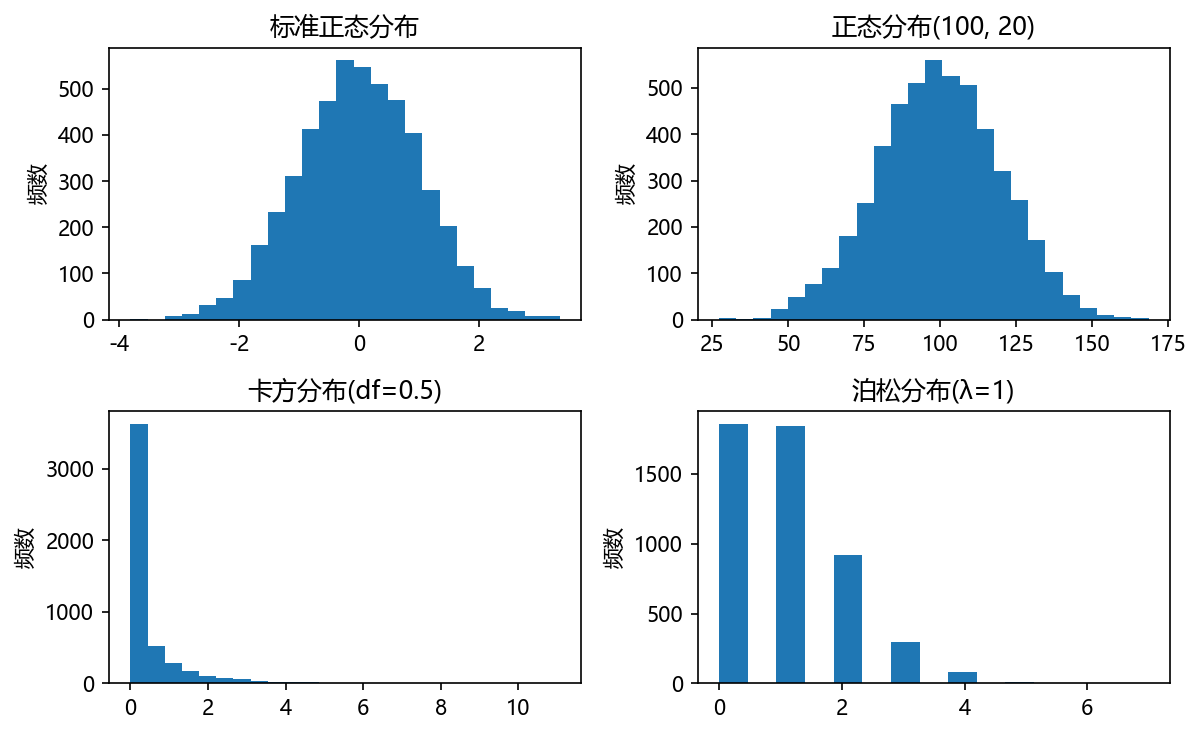
\includegraphics[width=0.85\textwidth]{mc_distributions}
	\end{center}
	\begin{itemize}
		\item 左上：标准正态（钟形对称）；右上：正态(100, 20)——形状相同、位置缩放不同。
		\item 左下：卡方分布（右偏、只取正值，用于利率模型）；
			右下：泊松分布（离散，模拟\alert{罕见冲击}发生的次数）。
	\end{itemize}
\end{frame}


%==============================================================
\section{模拟随机变量：一步到位}
%==============================================================

\begin{frame}{股价的"终点"长什么样}
	\begin{itemize}
		\item BSM 框架下，已知今天的股价 $S_0$，到期日 $T$ 的价格满足：
	\end{itemize}
	\begin{equation*}
		S_T = S_0 \exp\!\left(\left(r - \tfrac{\sigma^2}{2}\right)T
		+ \sigma\sqrt{T}\, z\right),
		\quad z \sim N(0,1)
	\end{equation*}
	\begin{itemize}
		\item $r$：无风险利率；$\sigma$：波动率；$z$：标准正态随机变量。
		\item 抽一个 $z$，就得一个可能的 $S_T$；抽一万个 $z$，
			就得到 $S_T$ 的\alert{整个分布}。
		\item $S_T$ 呈\textbf{对数正态分布}：恒为正、右偏（暴涨的可能性拖出长尾）。
	\end{itemize}
	\begin{alertblock}{零基础提醒}
		$\exp$ 就是指数函数 $e^x$（\texttt{np.exp}）。
		这个公式不用会推，\alert{会照着写代码}就行。
	\end{alertblock}
\end{frame}

\begin{frame}[fragile]{静态模拟：直接模拟到期日}
\begin{lstlisting}
S0, r, sigma, T = 100.0, 0.05, 0.25, 1.0   # 参数
I = 10000                                   # 模拟次数
np.random.seed(1000)
ST = S0 * np.exp((r - 0.5 * sigma ** 2) * T
         + sigma * np.sqrt(T) * npr.standard_normal(I))
ST.mean()   # 104.86
\end{lstlisting}
	\begin{itemize}
		\item 一行表达式模拟 10000 个到期价格——\textbf{向量化}的威力（第8章已见）。
		\item 理论均值 $S_0 e^{rT} = 105.13$，模拟得到 104.86——抽样误差之内，吻合。
	\end{itemize}
	\begin{center}
		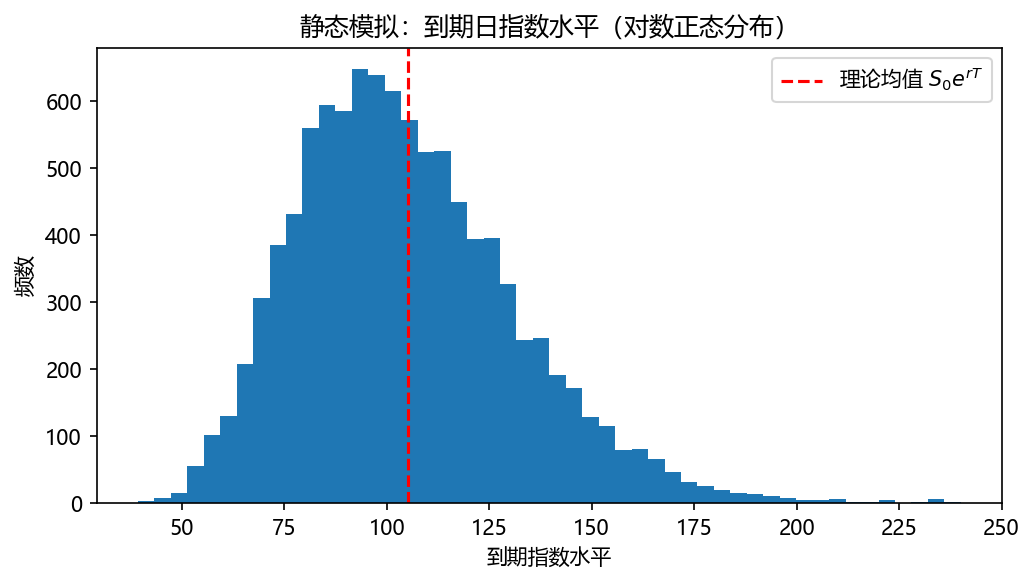
\includegraphics[width=0.55\textwidth]{mc_static_hist}
	\end{center}
\end{frame}

\begin{frame}{静态模拟的启示}
	\begin{itemize}
		\item 大部分路径落在 100 元附近，但右尾拖得很长：
			10000 条里最高冲到约 240 元，最低约 39 元。
		\item \alert{股价不会为负}（指数函数恒正）——对数正态分布的天然优点。
		\item 只关心到期日？静态模拟一步搞定。
			但期权若\textbf{中途}有特殊条款（如提前行权、触碰障碍），
			就必须知道\alert{整条路径}——下一节的动态模拟。
	\end{itemize}
\end{frame}


%==============================================================
\section{模拟随机过程：走出路径}
%==============================================================

\begin{frame}{从"终点"到"路程"}
	\begin{itemize}
		\item \textbf{随机过程}：一串前后关联的随机变量。股价逐日演化就是典型。
		\item 把一年切成 $M=50$ 小步，每步 $\Delta t = T/M$，逐步推进：
	\end{itemize}
	\begin{equation*}
		S_t = S_{t-\Delta t}\, \exp\!\left(\left(r - \tfrac{\sigma^2}{2}\right)\Delta t
		+ \sigma\sqrt{\Delta t}\, z_t\right)
	\end{equation*}
	\begin{itemize}
		\item 每一步抽\alert{新的}标准正态随机数 $z_t$，乘到当前价格上。
		\item 这种逐步推进的写法叫\textbf{欧拉离散化}——听起来高深，
			其实就是一个 for 循环。
		\item 马尔可夫性质：明天的价格只取决于今天的价格，
			与"怎么走到今天"无关（无记忆）。
	\end{itemize}
\end{frame}

\begin{frame}[fragile]{动态模拟：循环走时间，向量化走路径}
\begin{lstlisting}
M = 50                 # 时间步数
dt = T / M             # 每步长度
I = 10000              # 路径条数
np.random.seed(1000)
S = np.zeros((M + 1, I))   # (51, 10000) 的大数组
S[0] = S0                  # 所有路径从100出发
for t in range(1, M + 1):
    S[t] = S[t - 1] * np.exp((r - 0.5 * sigma ** 2) * dt
             + sigma * np.sqrt(dt) * npr.standard_normal(I))
\end{lstlisting}
	\begin{itemize}
		\item 循环只有 50 次（时间步），每步内部 10000 条路径\alert{一次算完}。
		\item \texttt{S[-1].mean()} 得到 104.60——与静态模拟、理论值一致。
	\end{itemize}
\end{frame}

\begin{frame}{一万条路径中的十条}
	\begin{center}
		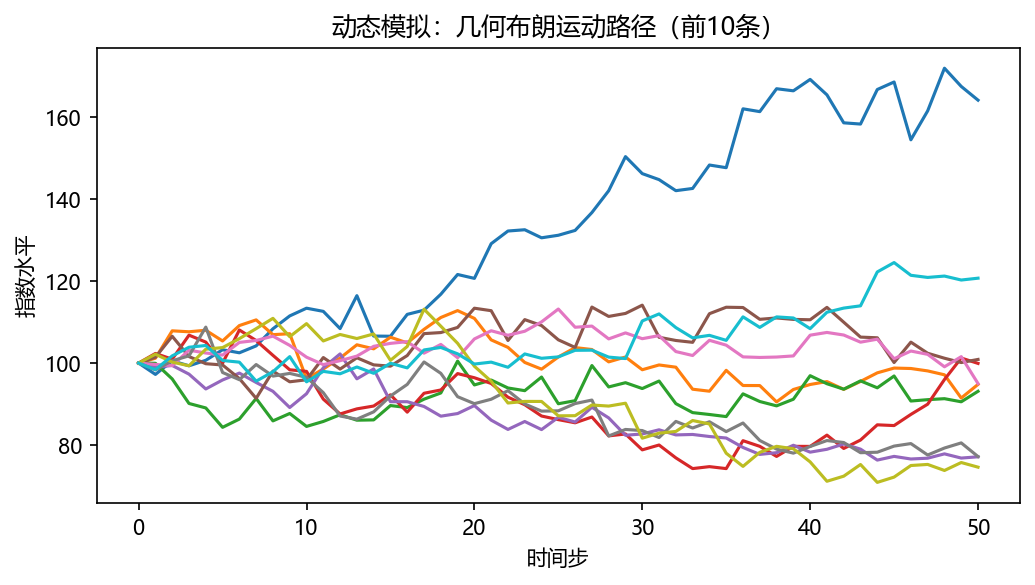
\includegraphics[width=0.72\textwidth]{mc_paths}
	\end{center}
	\begin{itemize}
		\item 每条路径都是"一种可能的未来"：有的一路向上，有的中途跳水。
		\item 动态模拟的额外收获：可以看清路径中途发生了什么，
			这是美式期权、障碍期权定价的基础。
	\end{itemize}
\end{frame}

\begin{frame}[fragile]{让随机数更"标准"：方差缩减}
	\begin{itemize}
		\item 之前看到：一百万个标准正态随机数的均值也不是精确的 0。
		\item 两招小手段可以强制达标：
	\end{itemize}
\begin{lstlisting}
sn = npr.standard_normal(5000)
# 技巧1：对偶变量——把相反数也加进来，均值必为0
sn = np.concatenate((sn, -sn))   # mean() = 0.0
# 技巧2：矩匹配——直接标准化，均值0、标准差1
sn = (sn - sn.mean()) / sn.std() # std() = 1.0
\end{lstlisting}
	\begin{itemize}
		\item 随机数的"前两个矩"（均值、标准差）摆正后，
			模拟结果的波动更小、更稳定——故称\textbf{方差缩减}。
	\end{itemize}
	\begin{alertblock}{零基础提醒}
		课堂上先建立直觉即可；实务中这两个技巧常与蒙特卡洛定价配套使用。
	\end{alertblock}
\end{frame}


%==============================================================
\section{欧式期权的蒙特卡洛估值}
%==============================================================

\begin{frame}{把"平均"变成代码}
	\begin{itemize}
		\item 风险中性定价公式的蒙特卡洛版本：
	\end{itemize}
	\begin{equation*}
		C_0 \approx e^{-rT}\cdot \frac{1}{I}\sum_{i=1}^{I} h\!\left(S_T^{(i)}\right),
		\quad h(S_T) = \max(S_T - K,\, 0)
	\end{equation*}
	\begin{itemize}
		\item 翻译成人话，一共三步：
	\end{itemize}
	\begin{block}{蒙特卡洛定价三步曲}
		\begin{enumerate}
			\item \textbf{模拟}：生成 $I$ 个到期价格 $S_T^{(1)},\dots,S_T^{(I)}$
			\item \textbf{算收益}：每条路径到期收益 $\max(S_T-K,0)$（没赚就是 0）
			\item \textbf{折现取平均}：$e^{-rT}\times$ 平均收益
		\end{enumerate}
	\end{block}
\end{frame}

\begin{frame}[fragile]{给看涨期权定价（静态模拟）}
\begin{lstlisting}
K = 105.0                  # 行权价
I = 50000                  # 模拟路径数
np.random.seed(100)
sn = npr.standard_normal(I)
ST = S0 * np.exp((r - 0.5 * sigma ** 2) * T
         + sigma * np.sqrt(T) * sn)          # 第1步：模拟
hT = np.maximum(ST - K, 0)                   # 第2步：收益
C0 = np.exp(-r * T) * np.mean(hT)            # 第3步：折现平均
print(C0)   # 9.9626
\end{lstlisting}
	\begin{itemize}
		\item BSM 解析公式给出 \alert{10.00}，模拟得到 9.96，
			误差仅 $-0.4\%$——五万条路径已经相当准。
		\item \texttt{np.maximum(ST - K, 0)}：到期价超过行权价才赚钱，否则收益为 0。
	\end{itemize}
\end{frame}

\begin{frame}[fragile]{动态模拟：看涨看跌一起估}
\begin{lstlisting}
def gbm_mcs_dyna(K, option="call"):
    S = np.zeros((M + 1, I)); S[0] = S0
    for t in range(1, M + 1):                # 逐步走路径
        S[t] = S[t-1] * np.exp((r - 0.5*sigma**2)*dt
             + sigma*np.sqrt(dt)*npr.standard_normal(I))
    if option == "call":
        hT = np.maximum(S[-1] - K, 0)        # 看涨收益
    else:
        hT = np.maximum(K - S[-1], 0)        # 看跌收益
    return np.exp(-r * T) * np.mean(hT)
\end{lstlisting}
	\begin{itemize}
		\item 实测（$I=50000,\ M=50$）：看涨 \alert{10.00}（解析 10.00），
			看跌 9.92（解析 9.88）。
		\item 欧式期权用动态模拟"绕了远路"，但这是以后给美式期权定价的\textbf{脚手架}。
	\end{itemize}
\end{frame}

\begin{frame}{模拟得越多，估计越准}
	\begin{center}
		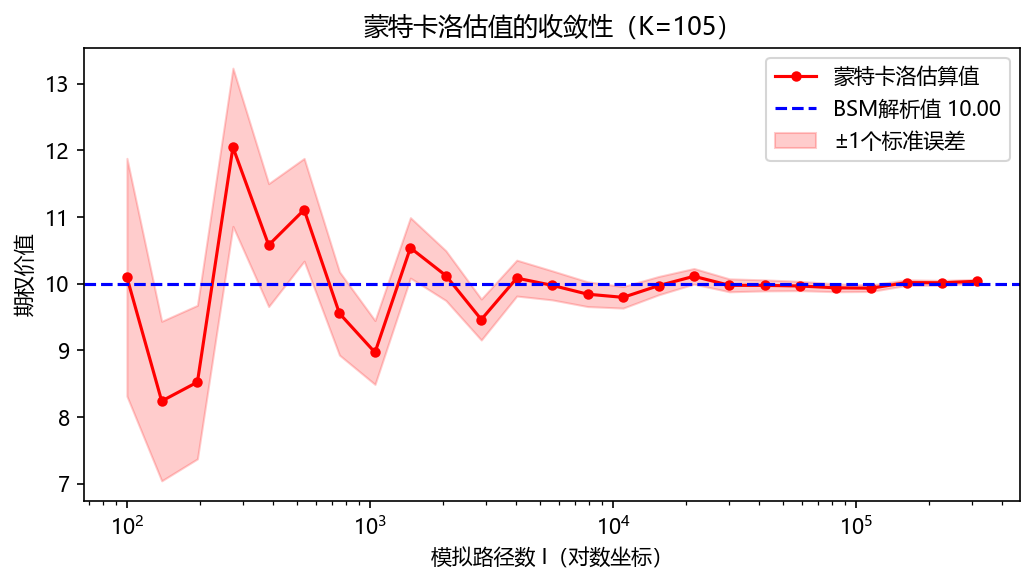
\includegraphics[width=0.68\textwidth]{mc_convergence}
	\end{center}
	\begin{block}{实测收敛过程（标准误差 = 标准差$/\sqrt{I}$）}
		\begin{tabular}{rcccc}
			\toprule
			路径数 $I$ & 500 & 5{,}000 & 50{,}000 & 500{,}000 \\
			\midrule
			估算值 & 10.35 & 9.94 & 9.97 & 9.97 \\
			标准误差 & 0.85 & 0.24 & 0.08 & 0.02 \\
			\bottomrule
		\end{tabular}
	\end{block}
	\begin{itemize}
		\item 误差按 $1/\sqrt{I}$ 缩小：\alert{精度提高 10 倍，样本要多 100 倍}——
			这就是蒙特卡洛"用算力换精度"的代价。
	\end{itemize}
\end{frame}

\begin{frame}{全面体检：一行权价范围对比}
	\begin{center}
		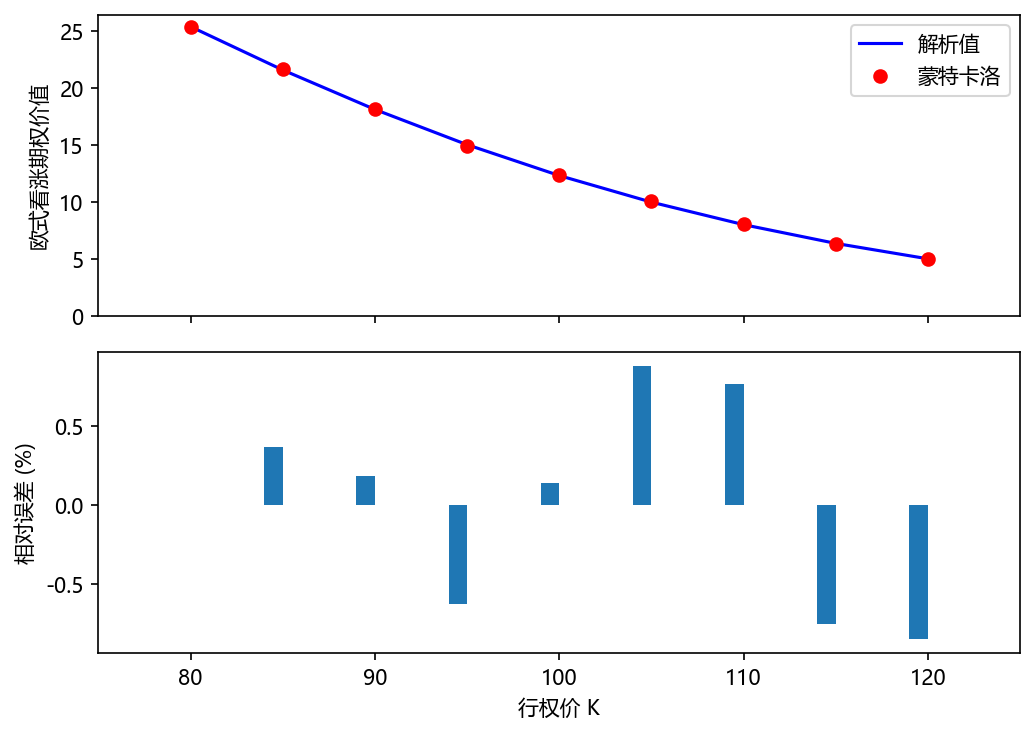
\includegraphics[width=0.72\textwidth]{mc_vs_analytic}
	\end{center}
	\begin{itemize}
		\item 行权价从 80 到 120，蒙特卡洛估算与解析值的\alert{最大相对误差不到 1\%}
			（实测 0.88\%）。
		\item 深度实值（K=80）与深度虚值（K=120）两端误差略大——
			收益分布越"偏"，需要的路径越多。
	\end{itemize}
\end{frame}


%==============================================================
\section{小结与练习}
%==============================================================

\begin{frame}{本章小结}
	\begin{itemize}
		\item \textbf{随机数}：\texttt{npr.seed} 保证可重现；
			\texttt{rand/standard\_normal} 是两大基础，
			线性变换可改变区间。
		\item \textbf{静态模拟}：一步模拟到期价格
			$S_T = S_0\exp((r-\sigma^2/2)T + \sigma\sqrt{T}\,z)$，对数正态分布。
		\item \textbf{动态模拟}：欧拉格式逐步推进，循环走时间、向量化走路径；
			是路径依赖产品定价的基石。
		\item \textbf{方差缩减}：对偶变量让均值精确为 0，矩匹配让标准差精确为 1。
		\item \textbf{蒙特卡洛估值}：模拟 $\to$ 算收益 $\to$ 折现取平均；
			误差按 $1/\sqrt{I}$ 收敛，与 BSM 解析值误差 $<1\%$。
	\end{itemize}
\end{frame}

\begin{frame}{课后任务与下章预告}
	\begin{block}{课后任务}
		\begin{enumerate}
			\item 用静态模拟估计\textbf{看跌期权}价值（收益为 $\max(K-S_T,0)$，
				$K=105$），并与解析值 9.88 对比。
			\item 把波动率从 0.25 提高到 0.40，重新定价看涨期权，
				观察价格变化方向并解释。
			\item 选做：分别用 $I=10^3, 10^4, 10^5, 10^6$ 条路径定价，
				记录标准误差，验证 $1/\sqrt{I}$ 规律。
		\end{enumerate}
	\end{block}
	\begin{exampleblock}{下章预告}
		本章的动态模拟写了一个时间循环——模拟一百万条路径时它够快吗？
		下一章讲 \textbf{性能}：为什么向量化比循环快，以及如何科学地计时。
	\end{exampleblock}
	\begin{center}
		\vspace{0.5em}
		本章内容改编自教材第12章\citep{hilpisch2018python}。
	\end{center}
\end{frame}


%==============================================================
%  附录：参考文献 + 结尾页
%==============================================================
\appendix

\begin{frame}[allowframebreaks]{参考文献}
	\bibliographystyle{style/gbt7714-2005}
	\bibliography{reference.bib}
\end{frame}

\begin{frame}
	\begin{center}
		{\Huge\calligra Thanks for your attention!}
		\vspace{1cm}

		{\Huge Q \& A}
	\end{center}
\end{frame}

\end{document}
